
\documentclass[aps,floatfix,prd,showpacs]{revtex4}
%\documentclass[aps,floatfix,prd,showpacs,twocolumn]{revtex4}
\usepackage{graphicx}% Include figure files
\usepackage{dcolumn}% Align table columns on decimal point
\usepackage{bm}% bold math
\usepackage{rotating}
 \usepackage{algpseudocode}
\voffset 1.0cm

\begin{document}


\title{Comparison of Computer Simulation Methods for Predicting Chemical Reactions}
\author{Graham Gibson}
\affiliation{
IBM,
Austin TX,
78723,
USA.}

\date{\today}

\begin{abstract}

In this paper we compare two primary methods of predicting basic organic chemistry reaction predictions. We analyze two types of models, an NLP based Neural Network and an agent based model. We compare and contrast the complexity, accuracy, and generalizability of both models as applied to predicting organic chemistry reactions. Two basic reaction mechanisms are explored, Elimination and Addition reactions.  These two mechanisms are simple but fundamental to the set of organic reactions, as many more complicated reactions use this mechanisms as intermediates.  We first verify the model on an alkene halogen addition reaction and then investigate the models generalizability to the elimination reaction. 


\end{abstract}
\pacs{PACS numbers go here. These are classification codes for your  research. See {\tt http://publish.aps.org/PACS/} for more info.}
\maketitle

\section{Introduction}

The problem of reliably predicting organic chemical reactions is vital in computation chemistry and biology. A model that is able to describe 3-dimension conformations of reactions would go a long way towards solving the more complicated protein folding problem. Finding such a solution would have extremely beneficial consequences in the area of targeted drug development and computational medicine. Such a solution would also drastically reduce drug development time and help eliminate clinical trail risk.

Traditional computational chemistry approaches have involved analyzing the potential energy surface of the atoms in the n-molecule system. The energy surface contains an array of parameters from 3-d cartesian coordinates, to electronegativity, to electron-electron repulsion. Finding the most likely product is equivalent to finding minima in the energy surface using tradition techniques like gradient descent. This method is often termed molecular dynamics . 
A second approach that is frequently taken is to go deeper into the reaction and look at the driving quantum mechanical principles that are at play. These methods use a combination of approximation techniques to guess the Hamiltonian of an atom and analytically solve for the orbital energy. This allows one to identify reactive orbitals very precisely. The two primary methods are called Hartree-Fock and Density Functional Theory. 
Although these approaches are invaluable in their description of the energy of chemical reactions, they are both quite complicated and computationally involved. The quantum mechanical approaches are extremely resource intensive as the involve the approximation of complicated integrals and matrix multiplications. It also appears that both methods are essentially overkill when trying predict the result of organic reactions. The reasoning behind this is that chemistry students begin studying reaction mechanisms and gain the ability to predict basic reactions long before they learn about solving Hamiltonian equations. Organic chemistry textbooks focus on what we call the "grammar" of organic chemistry. This involves  studying common reaction mechanisms and patterns of behavior of common functional groups such as OH, COOH, alkenes etc. Organic chemistry students learn chemistry as a combination of a language of interacting words and they verify reaction products as syntactically and semantically valid under such language. Using this view we can define two separate higher level approaches to predicting chemical reactions.

\subsection{First Approach: Language Based Modeling }
Continuing with the idea of modeling organic reactions as language over the alphabet of atoms, predicting a chemical reaction has a natural analogy between verifying if a sentence is valid in a given language. This problem has been studied in depth in the field of computer science and has been most successfully modeled by using recursive neural networks (RNNs) such as the Long Short Term Memory network architecture. This architecture maintains state of the neural network by copying the hidden state $H_{t-1}$ to the hidden state $H_{t}$ using a series of memory gates. LSTM networks have gained a lot of popularity in the computer science community for their ability to remember context from many time steps previous to the current because of this copying of hidden layer state. A common LSTM network approach to the problem of machine translation is depicted below as in \cite(-sequence-to-sequence-learning-with-neural-networks) 
\begin{figure}[ht]
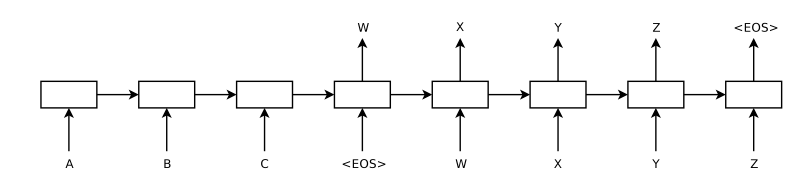
\includegraphics[width=7cm,angle=0]{fig1.png}
\caption{LSTM network feeding in an input sequence and target sequence.}
\label{fig1}
\end{figure}

This figure shows the input sequence being fed into the LSTM network one character at a time. In the chemistry analog we are feeding one atom in the textual representation of a molecule into the LSTM at a time step $t$.  As targets we feed the known product of a chemical reaction. Formally, we have:

$$ I = (i_1,i_2,...,i_n)$$   $$ O = (o_1,o_2,...,o_n)$$. 

The LSTM is able to learn a function $f: I \rightarrow O$  using standard stochastic gradient descent by first mapping the input and output character sets to one-hot encodings. If we examine a function $f$ produced by the neural network after an error threshold $e$ is reached we can investigate the semantic meaning of the mapping. The map $f$ takes input sequences of SMILES encoded reactants and outputs SMILES encoded products. For example 

$$ CCC=C \  \ HBr  \rightarrow CCCCBr$$

If we apply this function to variable length number of carbon off of the double bond we learn something about the function mapping. 

$$ f(CC_nC=C , \ HBr )\rightarrow CC_nCCBr$$
We see that the function $f$ has in a sense learned properties of the reaction. First, it knows that reactive site in the addition reaction is the alkene $C=C$ bond and is also able to understand that the number of $C$s is invariant under the mapping. \\




 \textbf{Results}

\begin{table}[ht]
\caption{Addition Reaction Learning after 50,000 Training Iterations}
\label{Addition}
\begin{tabular}{cclccl}
\hline
Input & Output &  Target & Correct\\
\hline
\hline
$CCCCCC=C \ HB$ & $CCCCCCCB$ & $CCCCCCCB$ & $Y$ \\
$CC=C \ HI$ & $CCCI$ & $CCCI$& $Y$  \\
$CCCCCCCCC=C \ HF$ & $CCCCCCCCCCF$ & $CCCCCCCCCCF$& $Y$  \\
$CC=C \ HF$ & $CCCF$ & $none$& $Y$ \\
$CC=C \ HCl $ & $CCCF$ & $none$& $N$ \\

\hline
\hline
\end{tabular}
\end{table}
As can be seen from $Table 1$ the map $f$ is able to learn that the number of $C$ atoms in the reactants and the products must be the same. However, the LSTM network was not able to abstract to halogens it has not seen before to understand that they behave in the same way. Unfortunately the last example highlights one of the greatest issues with neural network based approach for predicting chemical reactions. The neural network is only able to learn lexicographic similarities between inputs and targets and not chemical  similarities between training examples. The only way the network would have been able to correctly predict the last reaction is if it had previously seen the halogen in context of another reaction. In this way the neural network is learning the grammar of the chemical alphabet instead of the grammar of chemistry.
\\
\\
\textbf{Complexity}
\\
\\
Another issue of NLP neural network techniques is the size of the sample space. If we consider a reaction of two reactants whose strings are length $k_1$ and $k_2$ over an alphabet of size $n$ a randomly initialized neural network will produce strings with length between $(0, n^{k_1 + k_2})$. This space is much larger than the space derived from first principles which has size $m \choose 2$ where $m$ is the total number of atoms in the system.

\subsection{Second Approach: Agent Based Modeling }
Considering the limitations of the NLP approach described above we next turned to agent based modeling. Agent based models are comprised of multiple instantiations of classes of objects that are given objective functions. They are allowed to interact in a defined environment for a given number of time steps to improve their objective function. Agent based models have been used with a great deal of success to model complex behaviors that arise from a simple set of heuristics. There is also a very natural encoding from the chemical world to the ABM world. We define an agent as follows
$$A_i = (x, \ y, \ z, \ e, \ b, \ n)$$

Where $x,y,z$ are the standard cartesian coordinates, $e$ is the experimentally determined electronegativity of the element, $b$ is the maximal bond order for that given element, and $n$ is the set of agent linked to $A_i$. For example a carbon atom at the origin of the agent space is defined by,

$$C_i = (0, \ 0, \ 0, \ , 2.55, \ 4)$$

By defining an agent this way we can use two simple heuristics to update agent $A_i$ and agent $B_i$. Our global objective function is to maximize energetic stability of the system. We first let agents randomly move around a 3 dimensional cartesian coordinate and if the euclidean distance between agents $A_i$ and $B_i$ is within a sphere of radius $r$ they are allowed to interact. The two heuristics used to update agents are:\\

1) If $|A_i(n)| < A_i(b)$ and  $|B_i(n)| < B_i(b)$  then add $B_i$ to $A_i(n)$ and add $A_i$ to $B_i(n)$. 
\\rr
  2) If $|A_i(n)| < A_i(b)$ and $|B_i(n)| = B_i(b)$ and $B_i(e) < A_i(e)$  then set $B_i(n) =  {A_i}$
  
 This is equivalent to the two chemical statements:
 
  If agent $A_i$ can accept more bonds it will and if agent $B_i$ can accept more bonds it similarly will. 
  The second statement says that if a agent $A_i$ encounters an agent $B_i$ that has fulfilled its bond order, agent $B_i$ may still break its links to bond with agent $A_i$ if agent $A_i$'s electronegativity is greater. This is because bonds to elements with higher electronegativities are more stable. These two heuristics defined the bonding interaction between two agents but does not describe the geometric relationship between agents. This is handled by a separate heuristic determined by the principle of electron-electron repulsion. If we have agent $A_i$ with $|A_i(n)| > 2 $ then we need to define new $(x,y,z)$ coordinates for the neighbors that minimizes electron-electron repulsion. This can be done by a simple randomized algorithm :
  \begin{algorithmic}
  \State let $x,y,z$ be random in $R$
  
  \For{agent in $A_i(n)$ }
\If {$Volume(A_i(x)+x,A_i(y) + y,A_i(z) + z) >Volume(A_i(x),A_i(y),A_i(z))$  }
    \State $A_i(x) \gets A_i(x) + x$
     \State $A_i(y) \gets A_i(y) + y$
      \State $A_i(z) \gets A_i(z) + z$
\EndIf
\EndFor
\end{algorithmic}

\section{Conclusions}

Man, latex is great!

\acknowledgments
The author is grateful to Donald Knuth for inventing tex, and making publication quality typesetting a reality for scientists around the world.


\begin{thebibliography}{99}

\bibitem{lamport}
 {\sl LaTeX : A Documentation Preparation System User's Guide and Reference Manual}, Leslie Lamport [1994] (ISBN: 0-201-52983-1) pages: xvi+272.

\bibitem{latt}
I.M. Smart {\it et al.}, J. Plumb Phys. {\bf 50}, 393 (1983).

\end{thebibliography}

\end{document}



